% This Source Code Form is subject to the terms of the Mozilla Public
% License, v. 2.0. If a copy of the MPL was not distributed with this
% file, You can obtain one at http://mozilla.org/MPL/2.0/.
% 
%        Copyright 2018 Marco De Nicolo


\documentclass[11pt]{article}
\usepackage[utf8]{inputenc}
\usepackage{geometry}
\usepackage{graphicx} 
\geometry{a4paper} 
\usepackage{listings} % necessario per inclusione codice sorgente
\usepackage{color} % syntax highlighting
\usepackage{url}

\usepackage{amsmath}
\newcommand\ceil[1]{\lceil#1\rceil}
\usepackage{amsfonts}
\usepackage{amssymb}
\usepackage{pdfpages}
\usepackage{enumitem}

\definecolor{dkgreen}{rgb}{0,0.6,0}
\definecolor{gray}{rgb}{0.5,0.5,0.5}
\definecolor{mauve}{rgb}{0.58,0,0.82}

\lstset{frame=tb,
  language=python,
  aboveskip=3mm,
  belowskip=3mm,
  showstringspaces=false,
  columns=flexible,
  basicstyle={\small\ttfamily},
  numbers=none,
  numberstyle=\tiny\color{gray},
  keywordstyle=\color{blue},
  commentstyle=\color{dkgreen},
  stringstyle=\color{mauve},
  breaklines=true,
  breakatwhitespace=true,
  tabsize=3
}

\pdfinfo{
   /Author (Marco De Nicolo)
   /Title  (Documentazione Tecnica di Lost in Space)
}
\title{Documentazione Tecnica Progetto Basi di Dati\\Lost in Space}

\author{Marco De Nicolo\\ matricola: 871524\\ \url{marco.denicolo@studenti.unimi.it}}

\date{Gennaio 2018}

\begin{document}
\maketitle
\newpage
\section{Introduzione}
Lost in Space è un gioco di ruolo ambientato all'interno di una navicella spaziale.\\
Tutta la logica di gioco è stata implementata, con funzioni e trigger, all'interno della base di dati.\\
DBMS: Postgresql 10\\
Linguaggio procedurale all'interno della base di dati: PL/Python 3\\
Linguaggio back-end: Php 7\\
Linguaggi e meta-linguaggi lato client: HTML, CSS (dalla libreria Bootstrap3.3.6) e Javascript.\\
\section{Schema ER}
\begin{figure}[htp] \centering{
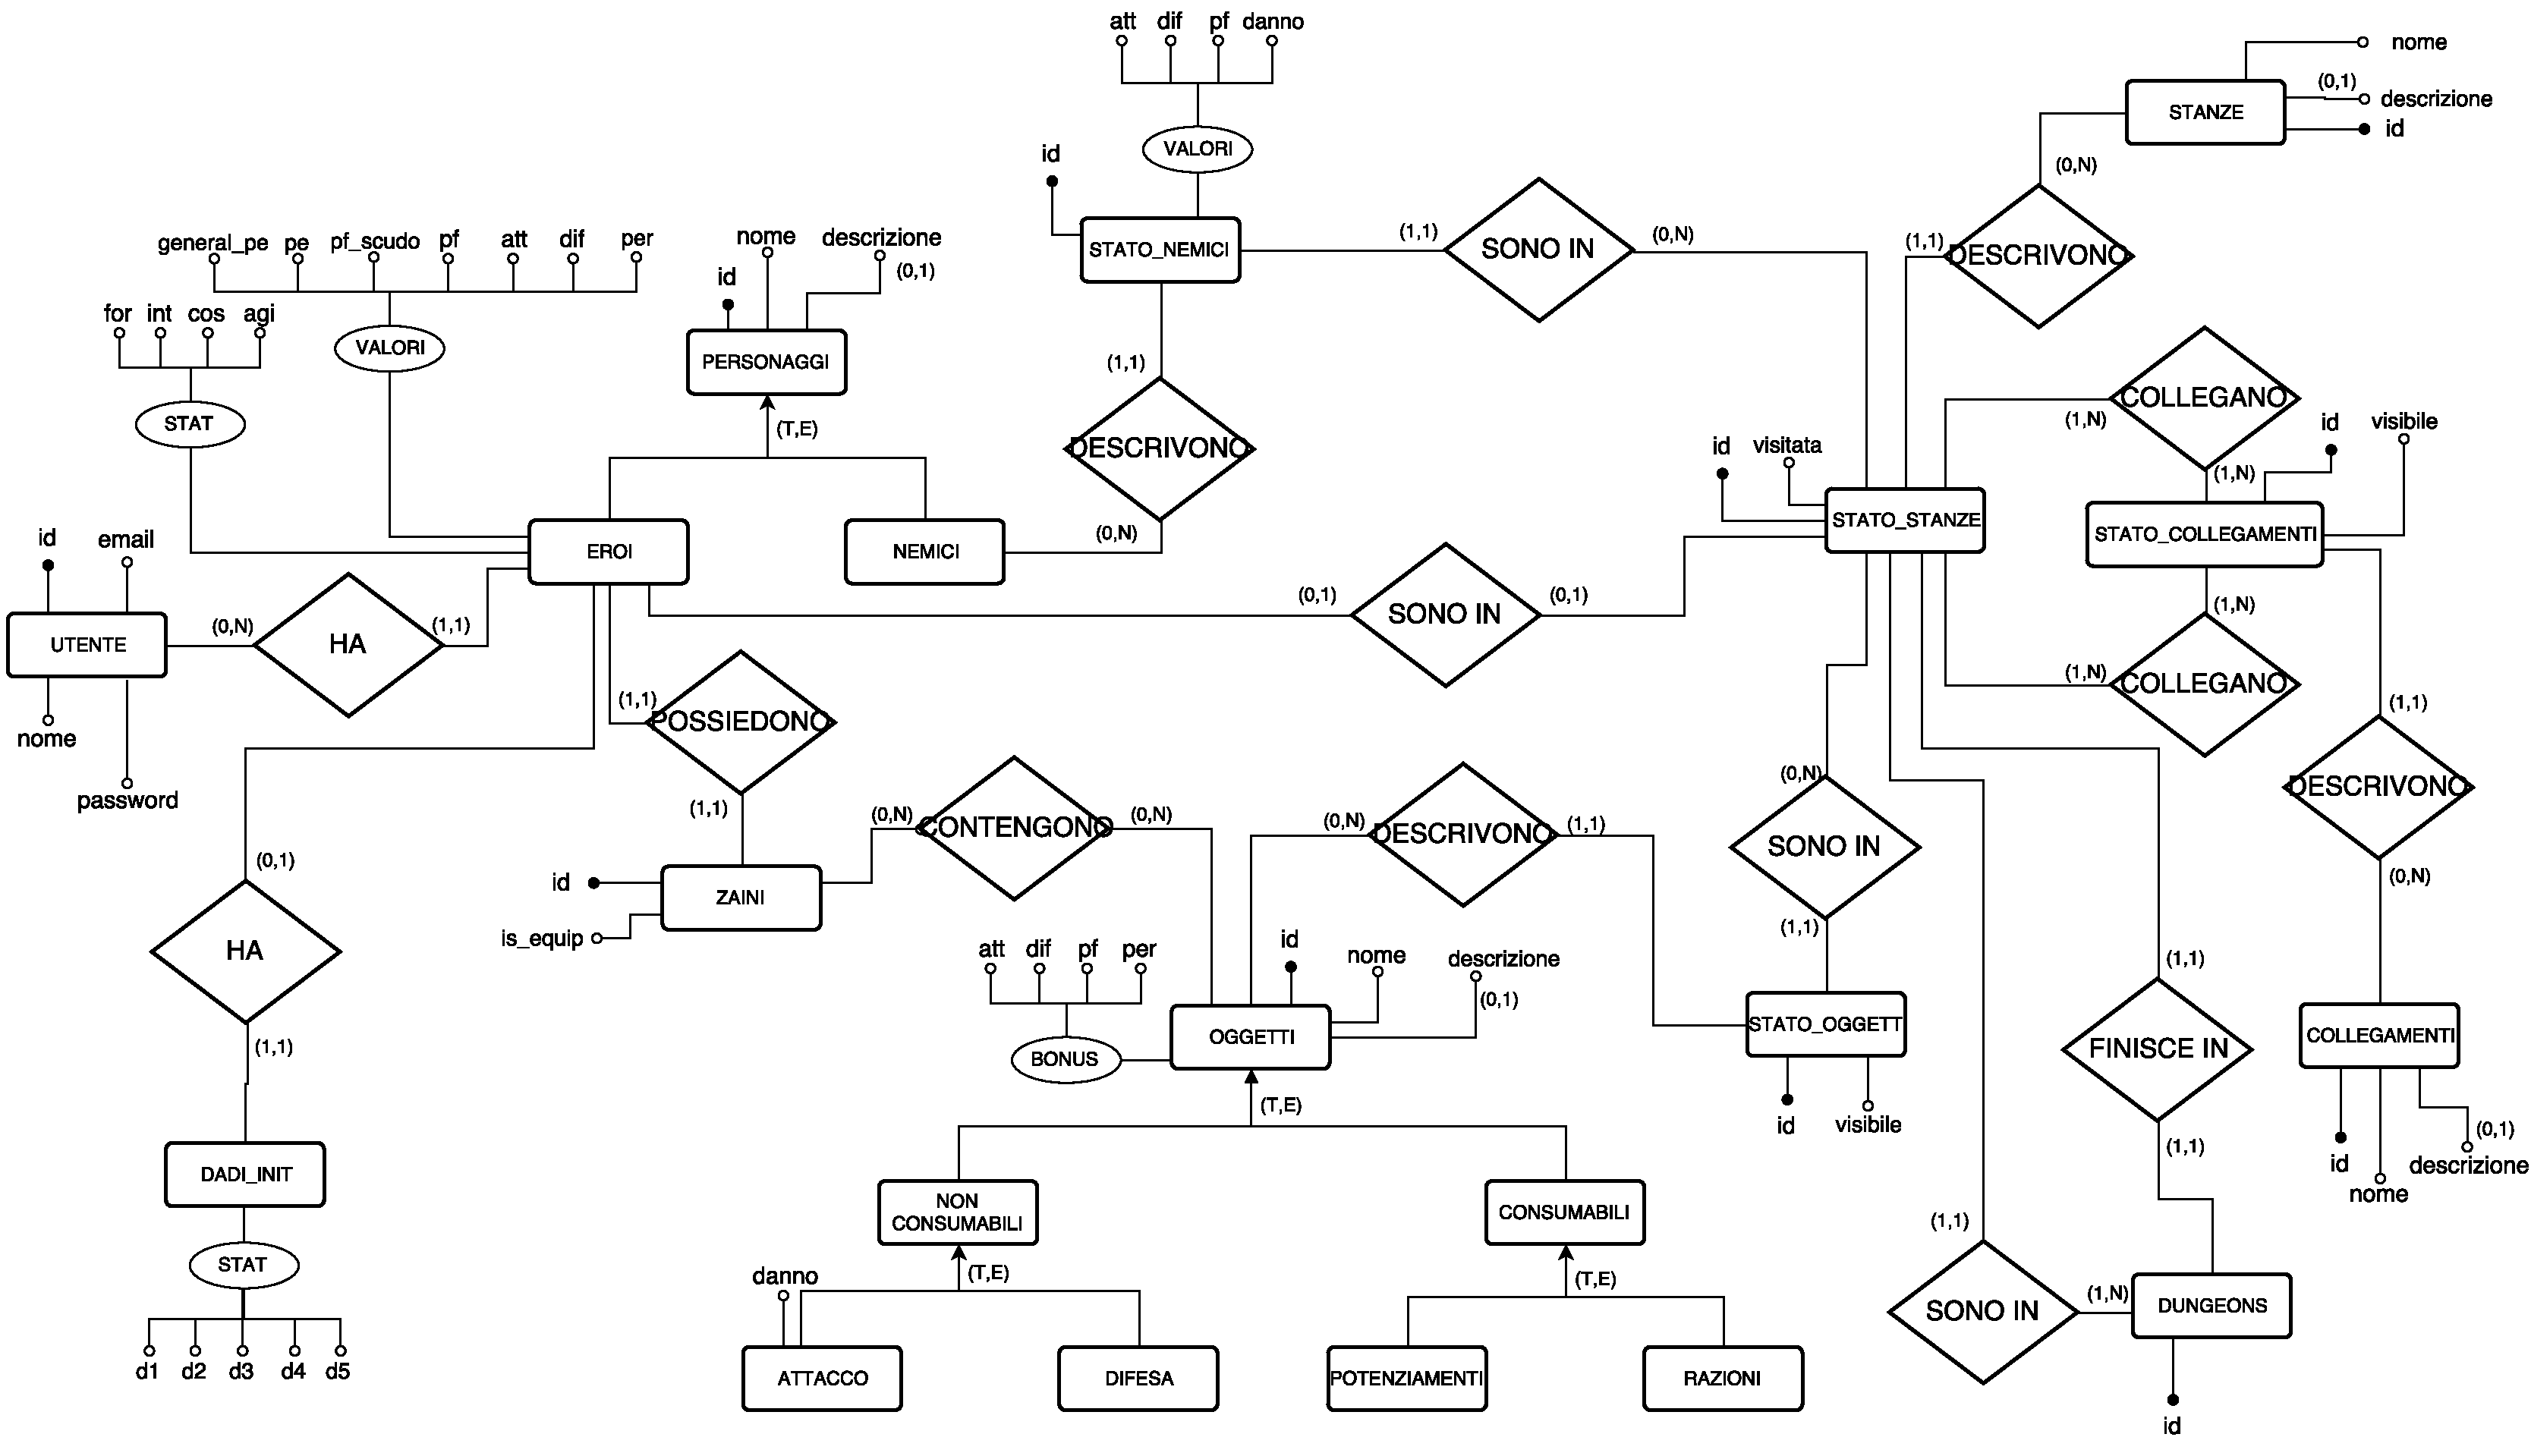
\includegraphics[scale=0.26]{progetto_bd.pdf}}
\end{figure}
\subsection{Osservazioni generali sullo schema ER}
Le entità che iniziano per "STATO\_" rappresentano l'entità che li descrive all'interno del dungeon, quindi, ad esempio, STATO\_NEMICI rappresenta i nemici esistenti in un dungeon e viene descritto da un'entità NEMICI.\\
DADI\_INIT viene usata nel momento della creazione del dungeon per salvare temporaneamente i valori del lancio dei dadi.\\
\section{Schema Relazionale}
\begin{itemize}
\item dadi\_init(\underline{\textit{id\_eroe}}, d1, d2, d3, d4, d5)
\item utenti(\underline{id}, mail, nome, password)
\item oggetti(\underline{id}, nome, descrizione*, att, dif, pf, per, danno, danno, tipo)
\item nemici(\underline{id}, nome, descrizione*)
\item stanze(\underline{id}, nome, descrizione*)
\item collegamenti(\underline{id}, nome, descrizione*)
\item eroi(\underline{id}, nome, descrizione*, forz, inte, cost, agil, general\_pe, att, dif, per, pf, pf\_scudo, pe, \textit{id\_sstanza*}, \textit{id\_utente})
\item dungeons(\underline{id}, \textit{finale})
\item stato\_stanze(\underline{id}, visitata, \textit{id\_stanza}, \textit{id\_dungeon})
\item stato\_collegamenti(\underline{id}, \textit{id\_from\_ss}, \textit{id\_to\_ss}, \textit{id\_collegamento}, visibile)
\item zaini(\underline{id}, \textit{id\_eroe}, \textit{id\_oggetto}, is\_equip)
\item stato\_oggetti(\underline{id}, \textit{id\_oggetto}, \textit{id\_sstanza}, visibile)
\item stato\_nemici(\underline{id}, att, dif, pf, danno, \textit{id\_nemico}, \textit{id\_sstanza})
\end{itemize}
\subsection{Traduzione da ER a Schema Relazionale}
Nella gerarchia totale-esclusiva dei personaggi tutti i campi sono stati portati alle entità figlie.\\
Nella gerarchia totale-esclusiva degli oggetti, invece, i campi dei figli sono stati portati all'entità padre ed è stato aggiunto un campo tipo(0: validi solo in stanza, 1: validi sempre (come le razioni), 2: attacco, 3: difesa).\\
Gli attributi composti BONUS, STAT e VALORE sono diventati singoli attributi separati.
\subsection{Domini}
I domini utilizzati nella base di dati sono:
\begin{itemize}
\item BONUS varia tra -6 e 6 ed è dato ai valori att, dif, pf e per degli OGGETTI
\item STATS varia tra 3 e 18 ed è dato ai valori d1, d2, d3, d4, d5 di DADI\_INIT ed ai valori forz, inte, cost, agil di EROI
\end{itemize}
\section{Funzioni e Trigger}
\subsection{Funzioni}
\subsubsection{CREATE OR REPLACE FUNCTION crea\_utente(nome TEXT, mail TEXT, upassword TEXT) RETURNS VOID}
Registra l'utente, la password viene salvata nella base di dati dopo aver usato una Key Derivation Function.
\subsubsection{CREATE OR REPLACE FUNCTION login\_utente(nomemail TEXT, upassword TEXT) RETURNS BOOLEAN}
Restituisce True se l'accesso va a buon fine, altrimenti false.\\Si può accedere con la mail o con il nome utente.
\subsubsection{CREATE OR REPLACE FUNCTION ini\_eroe(id\_utente INTEGER, nome TEXT, descrizione TEXT) RETURNS INTEGER}
Inizia la creazione dell'eroe inserendo nome,descrizione ed id\_utente.\\Restituisce l'id dell'eroe.
\subsubsection{CREATE OR REPLACE FUNCTION lancio\_dadi(id\_eroe INTEGER) RETURNS VOID}
Azzera lo zaino e tutti i valori dell'eroe, lancia 5 dadi per l'inizializzazione di DADI\_INIT.
\subsubsection{CREATE OR REPLACE FUNCTION fin\_eroe(id\_eroe INTEGER, forz TEXT, inte TEXT, cost TEXT, agil TEXT) RETURNS VOID}
Finisce la creazione dell'eroe inserendo i valori dei dadi che sono stati selezionati nelle rispettive caratteristiche.\\
Prima di ritornare elimina i valori utilizzati da DADI\_INIT
\subsubsection{CREATE OR REPLACE FUNCTION crea\_dungeon(id\_eroe INTEGER) RETURNS VOID}
Crea l'intero dungeon, composto da: stanze, collegamenti, oggetti e nemici.
Questo viene creato con un algoritmo che garantisce il collegamento tra tutte le stanze e che garantisce id sempre crescente da stanza iniziale a stanza finale.\\
Inizialmente creo per ogni stanza uno stato\_stanza, recupero gli id e li inserisco nella lista stati\_stanze, di seguito il resto dell'algoritmo:
\begin{lstlisting}
class Tree:
    def __init__(self):
        self.data = None
        self.child = []
.
.
.
stanze_prese = []
ind = len(stati_stanze)-1 #random.randint(0,len(stati_stanze)-1)
#sposto da stati_stanze a stanze_prese
root = Tree()
root.data = stati_stanze.pop(ind)
stanze_prese.append(root)
while(len(stati_stanze)>0):
    #a chi lo collego?
    ind = random.randint(0,len(stanze_prese)-1)
    val = stati_stanze.pop(-1)
    node = Tree()
    node.data = val
    stanze_prese[ind].child.append(node)
    stanze_prese.append(node)
    #creo il collegamento
    .
    .
    .
#inserisco stanza iniziale
inizio = find_start(root)[0].data
.
.
.
\end{lstlisting}
Prendo in ordine crescente gli id di stato\_stanze, li metto in un nuovo nodo che appendo casualmente nell'albero.\\
Il primo nodo che inserisco è root, la stanza finale.\\
find\_start fa una dfs dell'albero creato e mette come stanza iniziale quella con profondità maggiore.
\begin{lstlisting}
#funzione per cercare la stanza iniziale, prende un nodo del tree e ritorna un pair (nodo iniziale, profondita' maggiore)
def find_start(node):
    if len(node.child) <= 0:
        return [node,1]
    tupla = [None, 0]
    for n in node.child:
        t = find_start(n)
        if t[1] > tupla[1]:
            tupla = t
    tupla[1]+=1
    return tupla
\end{lstlisting}
In ogni stanza gli oggetti vengono inseriti casualmente, possono essercene da 0 a 6 tra visibili e non, infine aggiungo i due oggetti iniziali nello zaino dell'eroe.\\
Vengono aggiunti i nemici nelle varie stanze in modo che siano più deboli nelle prime stanze e più forti nelle ultime.
Prima di inserirli calcolo il range dei valori di att, dif, pf e danno considerando anche il massimo valore del bonus che l'eroe può ricevere da un oggetto, per ogni range calcolo l'incremento del valore per ogni stanza.
\begin{lstlisting}
#0<pEasy<=1, ad 1 e' piu' facile sconfiggere i nemici
pEasy = 0.3
#range delle stanze
rangeSs = len(stati_stanze_cp)-1
maxBonusAtt = plpy.execute("SELECT MAX(att) AS m FROM oggetti")[0]["m"]
#att = (for + agi)/2 + bonus, varia da 3 a 18+bonus, rangeAtt e' il range dell'attacco
rangeAtt = 18 + maxBonusAtt - 3
#calcolo l'incremento per ogni stanza, sottraggo un valore per semplificare il dungeon
incAtt = rangeAtt/rangeSs - pEasy*(rangeAtt/rangeSs)
\end{lstlisting}
\subsubsection{CREATE OR REPLACE FUNCTION adia\_stanza(sstanza INTEGER) RETURNS TABLE(id\_sstanza INTEGER, visibile BOOLEAN, nome\_stanza TEXT, visitata BOOLEAN, nome\_collegamento TEXT, descrizione\_collegamento TEXT)}
Restituisce una vista delle stanze adiacenti alla stanza passata come argomento.\\
Fa una ricerca su id\_from\_ss e id\_to\_ss della tabella STATO\_COLLEGAMENTI.
\subsubsection{CREATE OR REPLACE FUNCTION equip\_obj(id\_eroe INTEGER, id\_obj INTEGER, add BOOLEAN) RETURNS VOID}
Aggiunge i valori dell'oggetto passato ai valori dell'eroe se add è True, altrimenti li sottrae.\\
Questa funzione non aggiunge gli oggetti allo zaino, serve solo per incrementare o decrementare i valori dell'eroe.
\subsubsection{CREATE OR REPLACE FUNCTION attacco(id\_eroe INTEGER, id\_nemico INTEGER) RETURNS VOID}
Nella prima parte della funzione l'eroe attacca i nemici, nella seconda parte i sopravvissuti attaccano l'eroe.\\
Quando l'eroe uccide un nemico incrementa i suoi punti esperienza (pe) del valore "danno" del nemico.\\
L'eroe può proteggersi con uno scudo temporaneo utilizzando gli oggetti che lo potenziano una volta sola all'interno di una stanza.
\subsubsection{CREATE OR REPLACE FUNCTION segreti(id\_eroe INTEGER) RETURNS VOID}
L'eroe paga un pf o pf\_scudo per cercare oggetti o collegamenti nascosti nella stanza in cui si trova.
\subsection{Trigger}
\subsubsection{CREATE TRIGGER trigger\_capienza\_zaino BEFORE INSERT ON zaini FOR EACH ROW EXECUTE PROCEDURE capienza\_zaino();}
Prima di inserire un oggetto all'interno dello zaino si controlla il peso complessivo di questo e se supera $ \ceil{\frac{cost}{2}} $ non viene aggiunto.
\subsubsection{CREATE TRIGGER trigger\_reset\_e\_attacco AFTER UPDATE ON eroi FOR EACH ROW WHEN (OLD.id\_sstanza IS DISTINCT FROM NEW.id\_sstanza AND NEW.id\_sstanza IS DISTINCT FROM NULL) EXECUTE PROCEDURE reset\_e\_attacco();}
Quando l'eroe entra in una nuova stanza modifico questa come visitata.\\
Se é la stanza finale aggiorno i general\_pe, cancello il dungeon e chiamo la funzione lancio\_dadi per iniziare una nuova partita.
Se non è quella finale tolgo dallo zaino gli oggetti validi nella vecchia stanza e faccio attaccare i tutti i nemici della nuova stanza.
\subsubsection{CREATE TRIGGER trigger\_check\_type AFTER UPDATE ON zaini FOR EACH ROW WHEN (OLD.is\_equip IS DISTINCT FROM NEW.is\_equip AND NEW.is\_equip = 't') EXECUTE PROCEDURE check\_type();}
Dopo aver settato il valore is\_equip = True ad un oggetto nello zaino devono essere aggiornati i valori dell'eroe.\\
Se viene equipaggiato un secondo oggetto di tipo attacco o difesa si toglie quello vecchio per fare spazio a questo.\\
Se viene equipaggiato un oggetto di tipo 1, valido in tutto il dungeon, vengono aggiornati i valori dell'eroe e questo viene cancellato dallo zaino.\\
Viene richiamata la funzione equip\_obj per sommare o sottrarre i valori degli oggetti.
\subsubsection{CREATE TRIGGER trigger\_pf\_control AFTER UPDATE ON eroi FOR EACH ROW WHEN (NEW.pf \textless = 0 AND NEW.id\_sstanza IS DISTINCT FROM NULL) EXECUTE PROCEDURE pf\_control();}
Quando i pf dell'eroe sono minori o uguali a zero viene cancellato il dungeon e richiamata la funzione lancio\_dadi per resettare tutto e ricominciare una nuova partita.
\end{document}
